\section{Auswerung}

\subsection{Sättigungsdampfdruck und mittlere freie Weglänge}

Zunächst wird mit der Formel \ref{ps} der Sättigungsdampfdruck bestimmt.
Dafür wurden die verwendeten Temperaturen in Kelvin umgerechnet.
Für die verschiedenen Temperaturen ergeben sich folgende Werte für den Sättigungsdampfdruck p\textsubscript{sät} und die mittlere freie Weglänge $\bar w$:

\begin{minipage}{\linewidth}
    \begin{table}[H]
        \centering
    
    \begin{tabular}{lllll}
        \toprule
        Temperatur [$^\circ$C] & Temperatur [$^\circ$K] & p\textsubscript{sät} [mbar] & $\bar w$ & Verhältnis $\frac{a}{\bar w} $\\
        \midrule
        23  & 296,15 & $4.54 \cdot 10^{-3}$ & 6.39 $\cdot 10^{-3}$ & 1.57 \\
        155 & 428,15 & 5.83 & 4.97 $\cdot 10^{-6}$ & 2.01$\cdot 10^{3}$ \\
        181 & 454,15 & 14.6 & 1.98 $\cdot 10^{-6}$ & 5.04$\cdot 10^{3}$ \\
        \bottomrule
        
    \end{tabular}
    \captionof{table}{mitllere freie Weglänge und Vergleich mit dem Abstand Kathode-Beschleunigungselektrode}
    \label{tab:0}
    \end{table}
    \end{minipage}

\subsection{Differentielle Energieverteilung}

Um die differentielle Energieverteilung der Elektronen zu bestimmen muss zunächst die Skalierung der x-Achse bestimmt werden.
Dafür wurden beim Zeichnen der Kurven für die integrale Energieverteilung jeweils im Abstand von 1V eine Markierung auf dem Blatt gemacht.
Nun lassen sich die Abstände zwischen den Punkten bestimmen um eine Skalierung in V/mm zu erhalten. 1mm entspricht dabei einem Kästchen auf dem Papier.

\begin{minipage}{\linewidth}
    \begin{table}[H]
        \centering
    
    \begin{tabular}{lllll}
        \toprule
         & Abstände T= 23$^\circ C$ [mm] & Abstände T= 155$^\circ C$ [mm]\\
        \midrule
        0-1V  & 23 & 22     \\
        1-2V  & 21 & 22.5   \\
        2-3V  & 24 & 22.5   \\
        3-4V  & 21 & 23     \\
        4-5V  & 21.5 & 21.5 \\
        5-6V  & 22 & 23     \\
        6-7V  & 22 & 23     \\
        7-8V  & 21 & 23     \\
        8-9V  & 21.5 & 22.5 \\
        9-10V & 21 & 23     \\
        \midrule
        Mittelwerte & (21.8$\pm$0.95)mm & (22.6$\pm$0.49)mm \\
        Skalierung & (0.0459$\pm$0.002)V/mm & (0.0442$\pm$0.001)V/mm \\
        \bottomrule
        
    \end{tabular}
    \captionof{table}{x-Achsen Skalierungen für zwei verschiedene Energieverteilungen}
    \label{tab:1}
    \end{table}
    \end{minipage}

\noindent In der Tabelle \ref{tab:1} sind also die Abstände in Kästchen bzw. mm zu sehen. Aus diesen wurde der Mittelwert gebildet. Dabei entspricht derenungenauigkeit der Standardabweichung der Messwerte. Diese Mittelwerte geben zunächst an, dass 1V auf der x-Achse 21.8mm bzw. 22.6mm entsprechen. Die interessanteren Werte sind jedoch diejenigen, die angeben um wie viel Volt die Bremsspannung U\textsuperscript{a} größer wird, wenn sich 1mm nach rechts entlang der x-Achse bewegt wird. 
\noindent Um nun die differentielle Energieverteilung zu erhalten, werden wie in Abbildung ? und ? zu sehen Steigungsdreiecke eingezeichnet. Daraus kann die Steigung bestimmt werden. Wenn diese Steigungen gegen die Bremsspannung in einem Diagramm aufgetragen wird, ergibt sich die gesuchte differentielle Energieverteilung. Dabei sind die Steigungen proportional zur Anzahl der Elektronen und die Bremsspannung ist proportional zur kinetischen Energie der Elektronen. 

\noindent Die differentiellen Energieverteilungen sehen folgendermaßen aus:

\begin{figure}[H]
    \centering
    \includegraphics[height=8cm]{"8a1.png"}
\end{figure}

\begin{figure}[H]
    \centering
    \includegraphics[height=8cm]{"8a2.png"}
\end{figure}

Die aufgetragenen Werte sind in \ref{tab:3} und \ref{tab:2} zu finden.

\subsection{Franck-Hertz Kurve}

Auch in dieser Aufgabe muss zunächst die Skalierung der x-Achse bestimmt werden.
Dies geschieht analog zu der Vorgehensweise bei der Energieverteilung.


\begin{minipage}{\linewidth}
    \begin{table}[H]
        \centering
    
    \begin{tabular}{ll}
        \toprule
         & Abstände [mm]\\
        \midrule
        0-10V & 23 \\
        10-20V & 22 \\
        20-30V & 22.5 \\
        30-40V & 23 \\
        40-50V & 22.5 \\
        \midrule
        Mittelwert& (22.6$\pm$ 0.37)mm \\
        Skalierung& (0.44$\pm$ 0.007)V/mm  \\       
    \end{tabular}
    \captionof{table}{x-Achsenskalierung Franck-Hertz Kurve}
    \label{tab:5}
    \end{table}
\end{minipage}

\noindent Nun wird die erste Anregungsenergie benötigt. Diese ergibt sich, indem die Abstände der auftretenden Maxima mit der Elementarladung multipliziert werden.
Die Werte sehen wie folgt aus:

\begin{minipage}{\linewidth}
    \begin{table}[H]
        \centering
    
    \begin{tabular}{lll}
        \toprule
        Maxima & Abstände [mm] & Abstände [V]\\
        \midrule
        1-2 & 11 &   4.84 \\
        2-3 & 12 &   5.28\\
        3-4 & 11.5 & 5.06\\
        4-5 & 12 &   5.28\\
        5-6 & 12 &   5.28\\
        6-7 & 12.5 & 5.50\\
        7-8 & 12 &   5.28\\
        \midrule
        Mittelwert & & (5.22$\pm$0.19)V      
    \end{tabular}
    \captionof{table}{Abstände zwischen den Maxima der Franck-Hertz Kurve}
    \label{tab:4}
    \end{table}
\end{minipage}

\noindent Aus diesem Mittelwert ergibt sich die erste Anregungsenergie U\textsubscript{1} zu (5.22$\pm$0.19)eV

\noindent Um die Wellenlänge des emmitierten Lichts zu bestimmen wird folgende Formel verwendet:
\begin{equation}
    \lambda = \frac{h\cdot c}{E}
\end{equation}

\noindent Diese Gleichung ist eine Kombination aus:

\begin{align}
    \lambda = \frac{c}{f} \nonumber \\
    E = h \cdot f  \nonumber
\end{align}

\noindent Mit h = $4.136 * 10^{-15}$eVs und c =  $3*10^8$ m/s ergibt sich für die Wellenlänge:
\begin{displaymath}
    \lambda = 238\pm 9 nm
\end{displaymath}   

\section{Diskussion}

\subsection{allgemeines}

Die Auswertung dieses Versuchs ist durchaus fehlerbehaftet. Das liegt daran, dass die Messwerte alle aus gezeichneten Kurven abgelesen sind. Dabei entsehen Ablesefehler. Des Weiteren sind auch beim Zeichnen der Kurven ein paar Probleme aufgetreten wie zum Beispiel die Schwankung der Temperatur. Die Temperatur schwankte immer stärker je höher sie eingestellt wurde und unter anderem deshalb entstehen bei den Kurven, die unter hohen Temperaturen aufgenommen wurden keine glatten sondern leicht wellige Kurven. Dieser Umstand erschwert das Ablesen der Werte auch noch ungemein, was auch einen Fehler liefert. Das Bilden von Mittelwerten liefert auch noch Ungenauigkeiten. Diese sind aber so gering, dass der Fehler durch das Ablesen deutlich größer sein dürfte und die Fehler aus der Mittelwertbildung fast zu vernachlässigen sind.


\subsection{Sättigungsdampfdruck und mittlere freie Weglänge}

Es ist deutlich zu erkennen, dass bei steigender Temperatur der Sättigungsdampfdruck steigt und damit die mitlere freie Weglänge sinkt. Dies ist insofern sinnvoll, dass bei erhöhten Temperaturen sich die Hg-Atome schneller bewegen und es deshalb schneller zu stößen kommt.

\subsection{Energieverteilung}

Bei der differentiellen Energieverteilung fällt als erstes auf, dass der peak nicht infinitisimal breit ist. Das liegt daran, dass die Elektronen unterschiedlich große Energien beim Austritt haben. Dieses Phänomen wird als Fermi-Dirac-Verteilung bezeichnet. Bei RaumTemperatur haben die meisten Elektronen eine Energie von 7,36eV. Da die Elektronen mit 11V beschleunigt wurden, ergibt sich ein Kontaktpotential von K\textsubscript{1}= 3,64V. Die Energieverteilung bei 155$^\circ$C ist ganz anders verteilt, weil es durch die kürzere mitlere freie Weglänge zu deutlich mehr Stößen kommt als bei Raumtemperatur. Deshalb entsteht der Einbruch bei dieser Energieverteilung bereits bei ungefähr 1,58V (erste Anregungsspannung-Kontaktpotential).

\subsection{Franck-Hertz Kurve}

Die erste Anregungsenergie sollte bei 4,9eV liegen. Der gemessene Wert von 5.22eV hat dazu eine Abweichung von 6,5\%. Dieser Wert ist unter Betrachtung der genannten Messungenauigkeiten sehr genau bestimmt. 
Das emmitierte Licht liegt mit einer Wellenlänge von 238nm im Ultraviolett-Bereich. Dieser Wert ist auch sehr nah an dem Literaturwert von 253nm. Dies ist durch die geringe Abweichung der Anregungsenergie nicht verwunderlich.

\subsection{Energieverlust elastischer Stoß}
An dieser Stelle sei gesagt, dass der Energieverlust der Elektronen bei zentralen elastischen Stößen vernachlässigbar gering wird durch den großen Massenunterschied zwischen dem Hg-Atom und dem Elektron.

\section{Tabellen und Graphen}

\begin{minipage}{\linewidth}
    \begin{table}[H]
        \centering
    
    \begin{tabular}{lllll}
        \toprule
        Steigung & Bremsspannung [V]\\
        \midrule
        0.00  &  0.00  \\        
        0.00  &  0.46  \\        
        0.00  &  0.92  \\        
        0.00  &  1.38  \\        
        0.00  &  1.84  \\        
        0.00  &  2.30  \\        
        0.00  &  2.76  \\        
        0.00  &  3.22  \\        
        0.00  &  3.68  \\        
        0.00  &  4.14  \\        
        0.00  &  4.60  \\        
        0.00  &  5.06  \\        
        0.00  &  5.52  \\        
        0.40  &  5.75  \\        
        1.20  &  5.98  \\        
        1.60  &  6.21  \\        
        2.20  &  6.44  \\        
        2.80  &  6.67  \\
        4.60  &  6.90  \\
        6.00  &  7.13  \\
        7.20  &  7.36  \\
        3.80  &  7.59  \\
        1.60  &  7.82  \\
        0.30  &  8.28  \\
        0.00  &  8.74  \\
        0.00  &  9.20  \\
        0.00  &  9.66  \\
        0.00  &  10.12  \\
        \bottomrule
        
    \end{tabular}
    \captionof{table}{differentielle Energieverteilung T=23$^\circ C$}
    \label{tab:3}
    \end{table}
    \end{minipage}

    \begin{minipage}{\linewidth}
        \begin{table}[H]
            \centering
        
        \begin{tabular}{lllll}
            \toprule
            Steigung & Bremsspannung [V]\\
            \midrule
            1.50  &   0.00 \\
            1.50  &   0.44 \\
            1.40  &   0.88 \\
            1.40  &   1.32 \\
            1.20  &   1.76 \\
            1.00  &   2.20 \\
            0.70  &   2.64 \\
            0.40  &   3.08 \\
            0.10  &   3.52 \\
            0.10  &   3.96 \\
            0.10  &   4.40 \\
            0.10  &   4.84 \\
            0.10  &   5.28 \\
            0.10  &   5.72 \\
            0.10  &   6.16 \\
            0.10  &   6.60 \\
            0.10  &   7.04 \\
            \bottomrule
            
        \end{tabular}
        \captionof{table}{differentielle Energieverteilung T=155$^\circ C$}
        \label{tab:2}
        \end{table}
        \end{minipage}

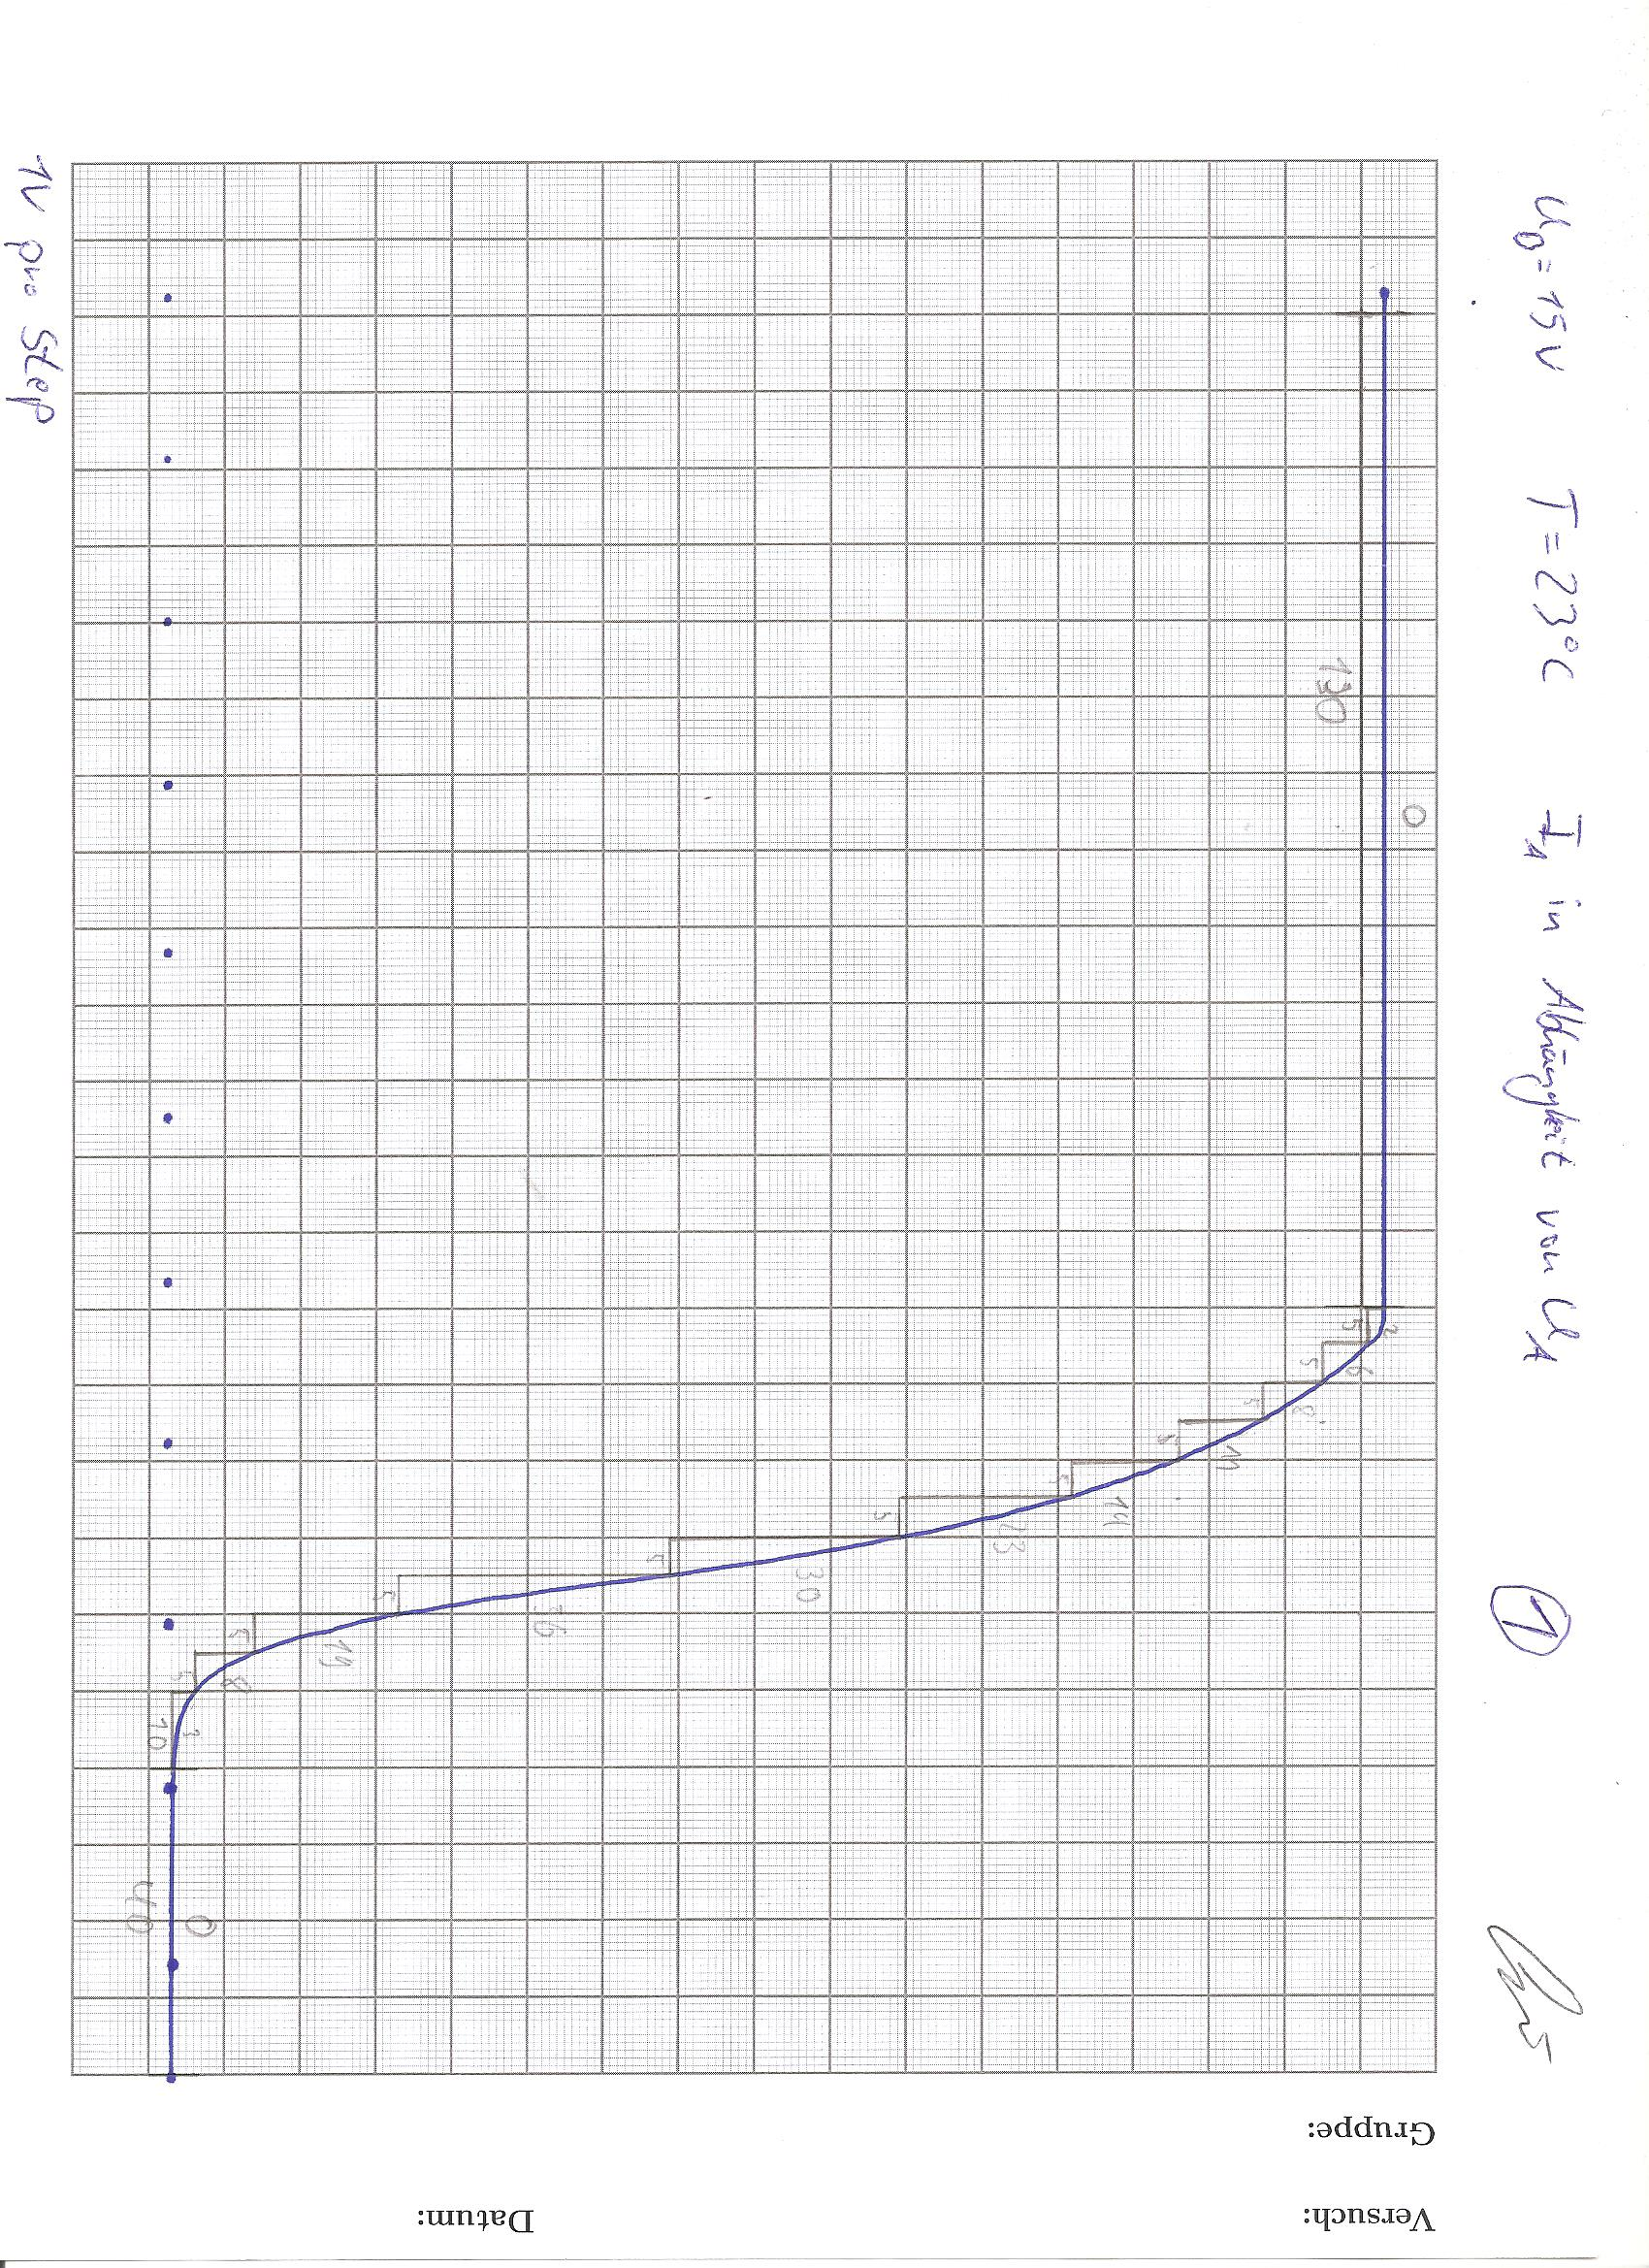
\includegraphics{Energieverteilung.jpg}

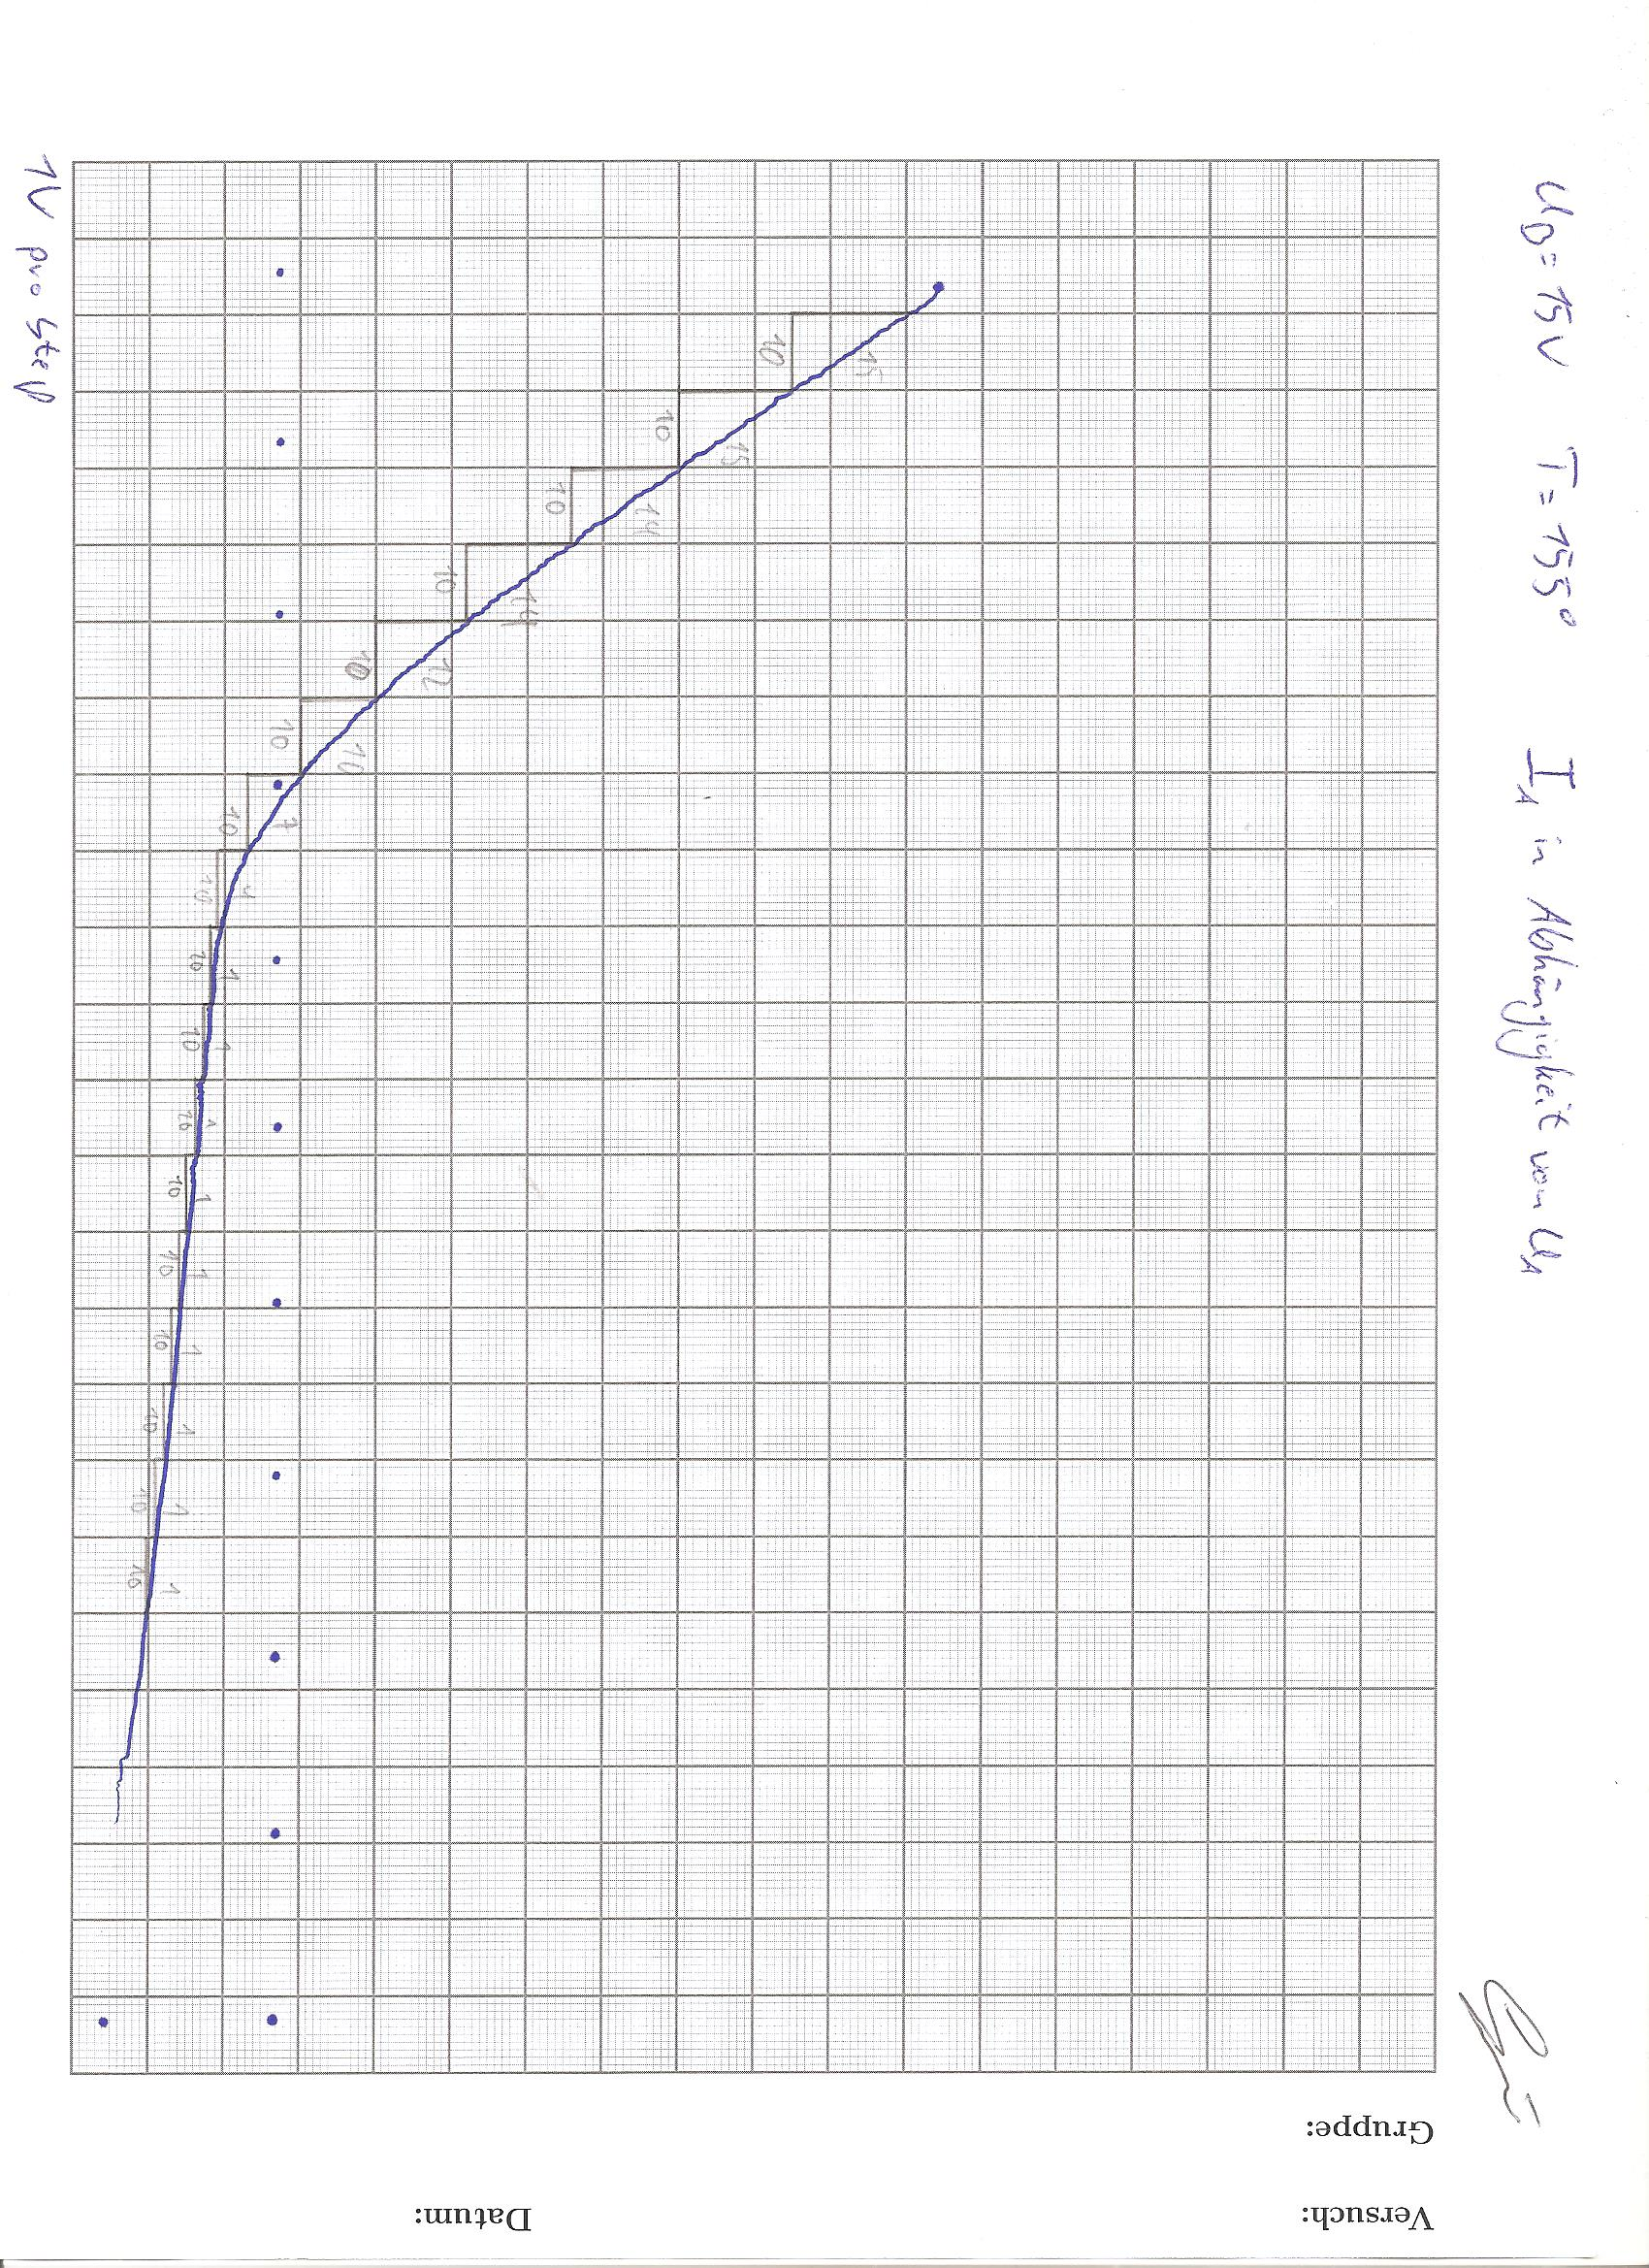
\includegraphics{Energieverteilung2.jpg}

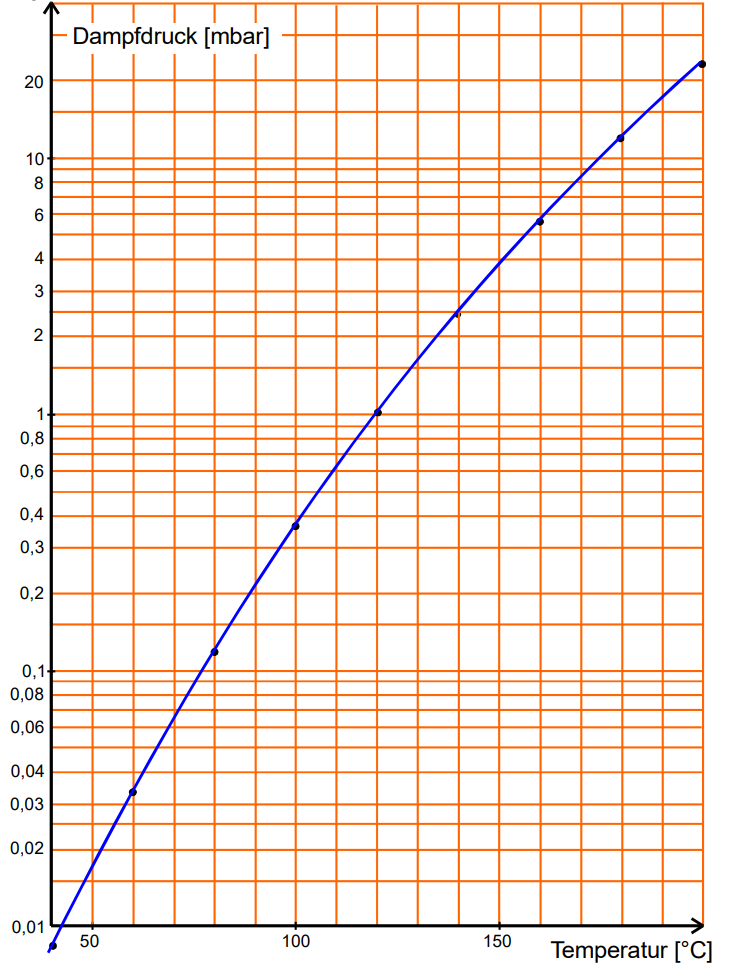
\includegraphics{Dampf_FranckHertz.png}